\documentclass[../manuale-sviluppatore.tex]{subfiles}

\begin{document}

\subsection{Plugin}

\subsubsection{Aggiunta di nuovi modelli di predizione}
All'interno del plugin, per gestire i diversi algoritmi di predizione dei dati, è stato utilizzato il design pattern Strategy come riportato nella seguente figura.

\begin{figure}[H]
  \centering
  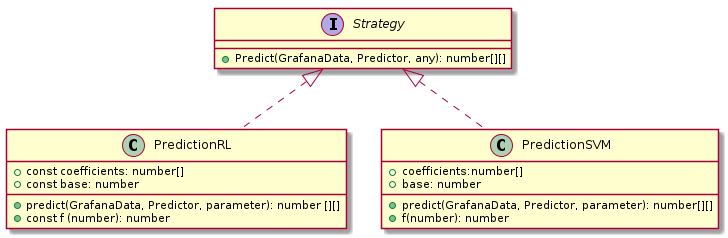
\includegraphics[width=15cm]{img/plugin/strategy.png}
  \caption{Strategy per la gestione degli algoritmi di predizione.}
\end{figure}

Dalla figura si possono notare le classi dei due algoritmi di predizione, ossia PredictionRL e PredictionSVM, con la stessa interfaccia comune Strategy.
Tali classi contengono al loro interno un metodo predict() che, ricevuti in input i valori sui quali effettuare la predizione e il parametro del predittore, restituiscono una matrice contenente i risultati della predizione. \\
Nel caso quindi si volesse includere un nuovo algoritmo di predizione dei dati i passaggi da svolgere per attuare tale cambiamento sono:
\begin{enumerate}
  \item Aggiungere una nuova Strategy, ossia la classe del nuovo algoritmo di predizione. Questa dovrà includere un metodo predict() con la stessa segnatura degli omonimi metodi degli algoritmi di predizione già implementati;
  \begin{figure}[H]
    \centering
    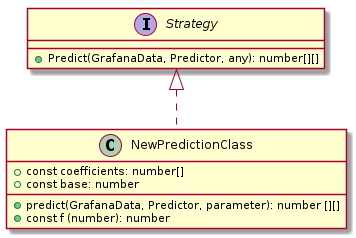
\includegraphics[width=10cm]{img/plugin/newstrategy.png}
    \label{fig:scice_documenti}
    \caption{Aggiunta di un nuovo algoritmo NewPredictionClass.}
  \end{figure}
  \item Aggiornare l'array associativo contenente l'identificativo degli algoritmi, aggiungendo l'id del nuovo algoritmo;
  \item Aggiungere il file di configurazione del nuovo algoritmo. Questo file conterrà i metodi propri di configurazione del nuovo algoritmo;
  \begin{figure}[H]
    \centering
    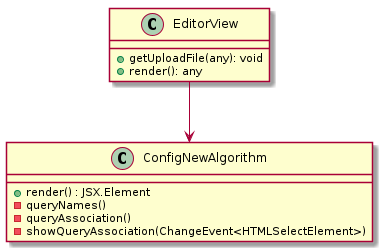
\includegraphics[width=10cm]{img/plugin/newconfig.png}
    \label{fig:scice_documenti}
    \caption{Aggiunta di una nuova configurazione ConfigNewAlgorithm.}
  \end{figure}
  \item Aggiornare l'array associativo contenente l'identificativo delle configurazioni degli algoritmi, aggiungendo l'id della configurazione del nuovo algoritmo.
\end{enumerate}


\end{document}
